\documentclass[10pt,a4paper,final]{article}
\usepackage[utf8]{inputenc}
\usepackage{amsmath}
\usepackage{mathtools, nccmath}
\DeclarePairedDelimiter{\nint}\lfloor\rceil
\usepackage{amsfonts}
\usepackage{amssymb}
\usepackage{float}
\usepackage{gitinfo2}
\usepackage{xcolor}
\usepackage[affil-it]{authblk}
\usepackage{comment}
\usepackage{pgfplots}
\usepackage{tikz}
\usetikzlibrary{datavisualization}
\usetikzlibrary{datavisualization.formats.functions}
\usetikzlibrary{patterns}
\usetikzlibrary{shapes.geometric,calc}
\usetikzlibrary{shapes.geometric,positioning}
\usetikzlibrary{shapes}
\usepackage[pdftex,
    pdfauthor={Adam Waldenberg, The Unigrid Foundation},
    pdftitle={Unigrid: A foundation for a decentralized, consensus-driven, segmented, blockchain-based Internet},
    pdfsubject={White Paper},
    pdfkeywords={blockchain;internet;bitcoin;unigrid;sharding;segmentation;consensus;decentralized;governance;gridnode},
    pdfproducer={Latex with hyperref, or other system},
    pdfcreator={pdflatex, or other tool}]{hyperref}
\usepackage[pdf]{graphviz}
\usepackage[automake]{glossaries}
\usepackage{bytefield}

\begin{comment}
\usepackage{xwatermark}
\end{comment}

\let\oldhref\href
\renewcommand{\href}[2]{\oldhref{#1}{\bfseries#2}}
\hypersetup{colorlinks = true, urlcolor = black, citecolor = black, linkcolor = black}
\author{\textit{Adam Waldenberg\\\href{mailto:adam@unigrid.org}{adam@unigrid.org}}}
\affil{The Unigrid Foundation\\\href{http://www.unigrid.org}{www.unigrid.org}}
\title{Unigrid: A foundation for a decentralized, consensus-driven, segmented, blockchain-based Internet}
\date{\emph{Draft Version \gitRel\hspace{5pt}(\gitCommitterDate)}}
\renewcommand*{\glstextformat}[1]{\textcolor{black}{\textit{#1}}}

\newcommand{\colorbitbox}[3]{%
  \rlap{\bitbox{#2}{\color{#1}\rule{\width}{\height}}}%
  \bitbox{#2}{#3}
}

\makeglossaries

\newglossaryentry{fermi}
{
	name=fermi,
	description={Smallest denomination of the Unigrid cryptocurrency, where one fermi is 0.00000001 units}
}

\newglossaryentry{gridnode}
{
	name=gridnode,
	description={Specialized service node providing the network with storage space, communication channels and compute cycles}
}

\newglossaryentry{shardgroup}
{
	name=shard group,
	description={A collection of \glspl{gridnode} servicing a unique blockchain to the network where wallets or daemons can store data. A shard group typically stores one shard, with other shards of the data being distributed onto other shard groups}
}

\newglossaryentry{unit}
{
	name=unit,
	description={Base currency unit and biggest denomination of the Unigrid cryptocurrency}
}

\begin{comment}
\newwatermark[allpages,color=red!15,angle=90,xpos=-85,ypos=0,scale=0.5]{CONFIDENTIAL UNTIL A LATER VERSION IS PUBLICLY PUBLISHED BY THE UNIGRID FOUNDATION}
\end{comment}

\begin{document}
\maketitle

\begin{abstract}
\noindent The original Internet was envisioned to become an open and distributed network that was scalable and fair, allowing access to data and services without surveillance or security concerns. However, in recent years, the network has become increasingly centralized and controlled by big businesses running huge data centers. This centralization has given big entities and businesses unprecedented control of the traffic and data of the network.
As a remedy to this deteriorating trend, we suggest the inception of a decentralized and consensus-driven segmented blockchain network based on a striped storage solution. The protocol allows for a completely decentralized and secure blockchain-based Internet where anybody, including private persons, can host an income-generating service node, aiding the network with compute cycles, bandwidth and storage space. To allow for complete utilization of the network, an access layer is provided, allowing for the development of protocols, services and infrastructure.
\end{abstract}

\section{Introduction}
During the last decade, the use of cryptocurrencies has increased dramatically with upward of 260 000 businesses now accepting cryptocurrency payments in Japan alone \cite{53companies2018}. Governments have enforced and expanded laws and policies in order to allow and promote continuous adoption \cite{japan2017}. While the Internet and the world moves towards an increasingly digitalized \cite{ekrona2019} and anonymized payment system pioneered by the Bitcoin network \cite{bitcoin2008} and its blockchain, the surveillance and control of the underlying Internet is continuously increasing on an annual basis, with servers and infrastructure moving into ever growing data centers controlled by big businesses. Private data is stored, controlled and distributed by these businesses - making the data centrally stored and inherently vulnerable. The public is, often unknowingly, placing private information and trust into these businesses, relying on them to store and keep the information and data safe and permanently secured. Not only does this control enable rogue entities to pressure businesses to release and disclose private information, but it also raises concerns related to the safe storage and longevity of the data itself \cite{guardian2017,facebook2018}. A partial solution is to use data encryption to secure and hide the information from prying eyes. This makes the data private, but the actual storage is in no way secured or guarantees longevity.

What is needed is a data storage solution that enables anybody to store and transmit data on the network in a distributed, secure and globally scalable way. If the network is designed to only allow individual nodes to have access to a small shard of any stored data, the network becomes more resilient against eavesdropping and attacks. If small shards are stored in different locations with redundancy employed in the form of striping, it creates a storage network where the data is spread out, making it completely resistant to local outages and external control.

The continuous centralization of the current Internet also causes congestion in the network, with many routes becoming almost completely obstructed during peak hours. A distributed network that globally stores data allows nodes to load balance the traffic of payloads and transmit data in many directions simultaneously.

Many cryptocurrency projects are maintained by commercial businesses that require steady funding and strict internal control of their underlying intellectual property. However, like with other infrastructure-providing digital solutions, historical data shows that open solutions are favoured for long-term sustainable adoption \cite{historyinternet2019,historybitcoin2019}.

To decrease central control and increase decentralization, the network employs decentralized sporks that allow service nodes to vote on changes and introduce modifications to the protocol of the network. All the properties of the protocol are either controlled or managed by the service nodes. Budget proposals, governance funding and service node collateral should all be controlled or managed in a decentralized fashion by the service node network and enforced by the board of The Unigrid Foundation.

\section{Gridnodes}
The former Darkcoin project originally developed the concept of masternodes aiding and providing the network with specific services \cite{darkcoin2014}. The Unigrid network takes this approach and develops it further into service nodes called \glspl{gridnode}. These specialized \glspl{gridnode} have the purpose of providing the network with storage space, communication channels and compute cycles. Ordinary network nodes and wallets communicating on the Unigrid network can send shards of work to the \glspl{gridnode}. Like transactions, sending these shards of work costs a certain amount of \glspl{unit} or \glspl{fermi}.

\subsection{Gridnode sporks}
Historically, network sporks have been controlled from a central controller and signed using spork keys in the possession of the project maintainers \cite{dashref2017}. While sporks are a useful feature that allows the network to toggle new network rules and control behaviour of the protocol, the fact that project maintainers can freely manipulate these sporks makes the solution centralized. If the spork key gets leaked or the maintainers are pressured into manipulating the network in a undesirable way, this creates a big security risk that can threaten the long-term viability of the network.

Unigrid completely ameliorates the spork system by introducing the concept of \gls{gridnode} sporks. \Gls{gridnode} sporks are either categorized as governed or ungoverned. While their concept is the same and the keys for signing these sporks are in the possession of The Unigrid Foundation, a governed \gls{gridnode} spork can only be modified after the \glspl{gridnode} on the network reach consensus and accept the change. Ungoverned \gls{gridnode} sporks, on the other hand, can be modified at will and are used by the developers of the system in order to tweak its behaviour for either performance considerations or testing. \Gls{gridnode} sporks also extend the definition of traditional sporks slightly. While normal sporks are defined as a single 64 bit number, \gls{gridnode} sporks have several fields while also defining a data portion for storing an arbitrary amount of data:

\bigskip
\begin{noindent}
	\begin{bytefield}[bitwidth=0.27em]{128}
		\bitheader{0, 63, 127} \\
		\bitbox{64}{timestamp}
		\bitbox{32}{data size}
		\bitbox{32}{delta size} \\
		\bitbox{64}{previous timestamp}
		\colorbitbox{lightgray}{64}{reserved} \\
		\begin{rightwordgroup}{data portion}
			\bitbox{16}{flags}
			\bitbox{16}{type}
			\colorbitbox{lightgray}{96}{reserved} \\
			\wordbox[lrt]{1}{spork data} \\
			\skippedwords \\
			\wordbox[lrb]{1}{}
		\end{rightwordgroup}
		\\
		\begin{rightwordgroup}{delta portion}
			\wordbox[lrt]{1}{spork delta data} \\
			\skippedwords \\
			\wordbox[lrb]{1}{}
			\vspace{0.25cm}
		\end{rightwordgroup}
	\end{bytefield}
\end{noindent}
\noindent The delta data stored in the \gls{gridnode} spork either contains the previous delta encoding, as described in section \ref{section:delta}, or the raw representation of the previous value of the spork. The flags section of the spork controls if the data stored in the delta portion is one or the other. Storing the previous timestamp and data in in this way allows the network to identify at what time a value was applied and, when requested, undo any recent change to a \gls{gridnode} spork. It also allows the network to undo a recent change to a governed \gls{gridnode} spork in the event that the change isn't accepted by the network. Furthermore, the \gls{gridnode} sporks defined in the protocol of the network are not static. As the network changes and evolves, governed and ungoverned \gls{gridnode} sporks can be continuously introduced and purged from the protocol in order to satisfy any changing requirements. \Gls{gridnode} sporks can only be added or removed to or from the protocol with new releases of the Unigrid daemon.

\subsubsection{Governed sporks}
Governed \gls{gridnode} sporks can modify the behaviour of the network to a greater extent than ungoverned \gls{gridnode} sporks and are therefore under strict network control and require consensus by the \glspl{gridnode} on the network before a change to them is accepted. The network defines a number of governed \gls{gridnode} sporks:

\begin{itemize}
\item \textbf{APPLY\_GRACE\_PERIOD} | Grace period defining the amount of time, in seconds, The Unigrid Foundation has to undo newly applied governed \gls{gridnode} sporks. This grace period is used by the network whenever the ungoverned \gls{gridnode} spork \emph{ROLLBACK\_SPORKS} is changed and allows the nodes on the network to verify which sporks should be reset back to their previous value.

\medskip
\begin{bytefield}[bitwidth=0.5em]{64}
	\bitheader{0, 31, 63} \\
	\bitbox{32}{grace period}
	\colorbitbox{lightgray}{32}{reserved}
\end{bytefield}

\item \textbf{SHARD\_GROUP\_REORGANIZE\_PERIOD\_INTERVAL} | Defines the minimum and maximum period, in seconds, that the ungoverned \gls{gridnode} spork \emph{SHARD\_GROUP\_REORGANIZE\_PERIOD} can be set to.

\medskip
\begin{bytefield}[bitwidth=0.5em]{64}
	\bitheader{0, 31, 63} \\
	\bitbox{32}{minimum period}
	\bitbox{32}{maximum period}
\end{bytefield}

\item \textbf{SHARD\_GROUP\_SIZE\_INTERVAL} | Controls the minimum and maximum value of the ungoverned \gls{gridnode} spork \emph{SHARD\_GROUP\_SIZE}.

\medskip
\begin{bytefield}[bitwidth=0.5em]{64}
	\bitheader{0, 15, 31, 63} \\
	\bitbox{16}{minimum size}
	\bitbox{16}{maximum size}
	\colorbitbox{lightgray}{32}{reserved}
\end{bytefield}
 
\end{itemize}

\subsubsection{Ungoverned sporks}
Several ungoverned \gls{gridnode} sporks are planned. These can be continuously changed by The Unigrid Foundation in order to fine-tune the network and modify its behaviour.

\begin{itemize}
\item \textbf{BLOCK\_REQUIRED\_COMPRESSION\_RATIO} | Sets the required compression ratio, as defined between 0 to 1. This defines how much compression is needed for the data portion of new blocks to be considered for storage at a \gls{gridnode} as a compressed block.

\medskip
\begin{bytefield}[bitwidth=0.5em]{64}
	\bitheader{0, 31, 63} \\
	\bitbox{32}{required ratio}
	\colorbitbox{lightgray}{32}{reserved}
\end{bytefield}

This only governs new blocks arriving at \glspl{gridnode}. If a block with an insufficient compression ratio is detected, the \gls{gridnode} should reject it. To enforce this rule, \glspl{gridnode} will randomly check blocks and heavily penalize nodes that break it by giving them a ban score, as describe in section \ref{section:penalties}.

\textbf{BLOCK\_VESTED\_ADDRESSES} | This spork defines a list of vested addresses and a single timestamp specifying when the vesting should begin. This is a spork used by The Unigrid Foundation to lock and manage sales of the Unigrid token. It is simply a list of addresses concatenated with the locked amount in each address together with the vesting period, the lock length and the creation timestamp. As the vesting schedule of the sale rounds proceeds, the network will allow for the continuous release of tokens held by these addresses.

\medskip
\begin{bytefield}[bitwidth=0.5em]{64}
	\bitheader{0, 31, 63} \\
	\bitbox{32}{timestamp vesting start}
	\colorbitbox{lightgray}{32}{reserved} \\
	\wordbox[lrt]{1}{address data} \\
	\skippedwords \\
	\wordbox[lrb]{1}{}
\end{bytefield}

The timestamp of this spork is initially empty, once the time has been set once, the daemon will never accept any additional changes to this spork. This limitation is put in place in order to make sure that this spork can not be abused in future versions of the daemon.

\item \textbf{ROLLBACK\_SPORKS} | When set to true, triggers a network-wide undo signal that rolls back recent spork changes.

\medskip
\begin{bytefield}[bitwidth=0.5em]{64}
	\bitheader{0, 1, 63} \\
	\bitbox{1}{}
	\colorbitbox{lightgray}{63}{reserved}
\end{bytefield}

Any \gls{gridnode} spork changed within the time of the grace period as defined by \emph{APPLY\_GRACE\_PERIOD} will be rolled back and assigned the previous timestamp and value as defined by \emph{previous timestamp} and \emph{previous value}. After the rollback, \emph{previous timestamp} and \emph{previous value} are set to \emph{NULL} and zero.

\item \textbf{SHARD\_GROUP\_REORGANIZE\_PERIOD} | Controls the reorganize period of shard groups. This is the interval at which a shard group should reorganize and compact the blockchain. This allows it to remove stale or in some other way invalid blocks from the chain.

\medskip
\begin{bytefield}[bitwidth=0.5em]{64}
	\bitheader{0, 31, 63} \\
	\bitbox{32}{period}
	\colorbitbox{lightgray}{32}{reserved}
\end{bytefield}

If the size is set to a value outside the allowed interval, the value is clamped accordingly to keep it within the required range as defined by the governed \gls{gridnode} spork \emph{SHARD\_GROUP\_REORGANIZE\_PERIOD\_INTERVAL}.

\item \textbf{SHARD\_GROUP\_SIZE} | Defines the preferred size of shard groups on the network. While the spork value sets the preferred size of shard groups, the network does not guarantee that a given shard group is of the requested size at any given time.

\medskip
\begin{bytefield}[bitwidth=0.5em]{64}
	\bitheader{0, 15, 63} \\
	\bitbox{16}{size}
	\colorbitbox{lightgray}{48}{reserved}
\end{bytefield}

If the size is set to a value outside the allowed interval, the value is clamped accordingly to keep it within the required range as defined by the governed \gls{gridnode} spork \emph{SHARD\_GROUP\_SIZE\_INTERVAL}.

\item \textbf{SHARD\_GROUP\_PARITY\_WEIGHT} | Defines the weight modifier for the parity calculation in the striping algorithm as defined by figure \ref{fig:parityweight}. The resulting calculation is hard-coded to be clamped between 0.1 and 0.3, meaning this unmanaged \gls{gridnode} spork lacks any managed spork(s) controlling it.

\medskip
\begin{bytefield}[bitwidth=0.5em]{64}
	\bitheader{0, 31, 63} \\
	\bitbox{32}{weight}
	\colorbitbox{lightgray}{32}{reserved}
\end{bytefield}
\end{itemize}

\subsubsection{\Gls{gridnode} spork consensus}
While ungoverned \glspl{gridnode} sporks can be modified freely by The Unigrid Foundation, the governed \gls{gridnode} sporks have to be accepted by the network. By default, if a \gls{gridnode} does not reject the proposal to change a value, it will automatically accept it. Whenever a governed \gls{gridnode} spork is modified by the foundation, the network collects \emph{VOTE} blocks (\ref{block:vote}) and counts the number of rejections passed from gridnodes. The new value is then either accepted or rejected by the network based on the outcome.

\subsection{Dynamic collateral adjustment}
\label{section:dyncol}
The collateral is the minimal amount of Unigrid tokens required to deploy a \gls{gridnode} on the network. A \gls{gridnode} and its collateral is deployed to the network by registering a public \gls{gridnode} key and associating it with a transaction ID on the network. This is similar to how traditional masternodes are implemented \cite{darkcoin2014}.

In order to facilitate organic growth, the Unigrid network employs a dynamic collateral adjustment. This means that the minimum collateral needed for a \gls{gridnode} decreases with the growth of the network and continuous addition of new \glspl{gridnode}. The network will always accept larger amounts - operators are therefore never forced to reorganize their nodes on each level-change;

\[
	\left\{
		\begin{array}{l}
		c_1 = 3000\\
		c_n = \nint*{ c_{n - 1} - c_{n - 1} \times 0.025 \times \log c_{n - 1}^{(5 - 0.1  \times n) \vee 1} }\\
		\end{array}
	\right\}
\]

\noindent The calculation runs for every additional 500 \glspl{gridnode} added to the network. Once the collateral level has progressed, it will never return to a previous level. Using the above recursive function we can calculate the required collateral at various adoption levels on the network;

\[
	\begin{array}{l}
	c_1 = 3000\\
	c_{10} \approx 718\ (5\ 000\ \glspl{gridnode})\\
	c_{30} \approx 138\ (15\ 000\ \glspl{gridnode})\\
	c_{50} \approx 80\ (25\ 000\ \glspl{gridnode})\\
	c_{100} \approx 33\ (50\ 000\ \glspl{gridnode})
	\end{array}
\]

\subsection{Scoring and rewards}
\label{section:scoring}
The \gls{gridnode} rewards on the Unigrid network retain the original reward structure originating from new block generation, where the calculation for the winning node uses a pseudo-random deterministic algorithm similar to the one described in the original Darkcoin specifications \cite{darkcoin2014}. This retains a flat and evenly distributed reward system for all the \glspl{gridnode} on the network.

As a complement, \glspl{gridnode} on the Unigrid network also receive rewards based on the services they provide. The nodes on the network are required to provide services such as bandwidth, domain name registrations, compute cycles and storage space. Each \gls{gridnode} is scored by individual wallets and daemons based on link speed, responsiveness, storage space and compute capacity.

\subsubsection{Bandwidth scoring}
Bandwidth scoring is based on link responsiveness and the ability to rapidly handle data transfers. A more responsive and faster uplink will result in the \gls{gridnode} receiving a higher score for the provided service;

\[
	\begin{array}{l}
	s_{br} = 100 \times \cfrac{1}{\log t_{ms}}\\
	s_{bs} = \cfrac{\frac{b^2}{t_s}}{1024}
	\end{array}
\]

\medskip
\noindent The score calculation independently keeps track of responsiveness and speed, where $s_{br}$ is the calculated responsiveness score and $s_{bs}$ is the calculated speed score. The time in milliseconds to receive a response to a request is denoted by $t_{ms}$. The number of transfered bytes is denoted by $b$ with the time taken for a transfer in seconds denoted by $t_s$.

\subsubsection{Compute scoring}
Peers calculate the compute performance by comparing \glspl{gridnode} against members of the same \gls{shardgroup}. Every other time a \gls{shardgroup} receives a compute block it will either assign the block to the highest scoring \gls{gridnode} or randomly send the block to three unique members of the \gls{shardgroup}. If sent to multiple members, each \gls{gridnode} receives a score for their attempt;

\[
	\begin{array}{l}
	s_{a_{_C}}, s_{a_{_G}} = \left( \cfrac{1}{\frac{t_a}{\frac{t_b + t_c}{2}}} \right) ^2\\
	\end{array}	
\]

\noindent This calculation is repeated for each of the three selected \glspl{gridnode} and ensures a fair distribution of work, where the faster nodes are given a better score and higher resulting priority. The time in milliseconds to complete a compute block for each node is denoted by $t_{a}$, $t_{b}$ and $t_{c}$. The resulting score $s_{a}$ is the score for the \gls{gridnode} that took $t_{a}$ milliseconds to complete the block. Every completed compute block type (CPU or GPU) is separately calculated as denoted by $s_{a_{_C}}$ and $s_{a_{_G}}$.

\subsubsection{Score deduction}
Whenever a \gls{gridnode} is assigned work, the score of that \gls{gridnode} is decreased by the total score of that work, as calculated and described in section \ref{section:scoring}. This results in a \gls{shardgroup} that constantly changes and reorders its member nodes as work is sent into the \gls{shardgroup} by nodes consuming their service.

\subsubsection{Scoring consensus and penalties}
\label{section:penalties}
When a \gls{shardgroup} receives work from a node, it is processed, executed or generally handled by a selected \gls{gridnode} with the highest score. However, another \gls{gridnode} will randomly re-send incoming work and calculate an intermediate score. This extra step is randomly done to prevent tampering and manipulation of the scoring algorithm. A node reporting a score that, as measured by the \gls{gridnode} is obviously manipulated will receive a misbehaviour score. If the offences continue, the node will collect enough misbehaviour points to be banned on the network.

\section{Dynamic rewards and exhaustion}
\label{section:dynreward}
The Unigrid network uses a naive approach to adjust the rewards that \glspl{gridnode} receive when they perform work for the network - allowing the network to democratically adjust the reward structure. The network does not allow \glspl{gridnode} to control how much they want to get rewarded for their services. Instead, the nodes collectively adjusts rewards based on the amount of available resources on the network and the current minting rate in new blocks.

\begin{figure}[htb]
	\centering
     \begin{tikzpicture}[baseline,remember picture, scale=1.3]
                \datavisualization [
                        scientific axes,
                        x axis = {label={\emph{reward modifier}}, length=5cm},
                        y axis = {label={exhaustion level}},
                        visualize as smooth line=three,
                        three={style={orange}}
                        ]
		                data [set=three, format=function] {
	    		            var x : interval [-1:1];
    	        		    func y = (pow(\value x, 3) + 1) * 0.5;
		                };
        \end{tikzpicture}
		\caption{Describes how the exhaustion level on a \gls{gridnode} influences the reward modifier that the network and the nodes use as a baseline for its reward decisions.}
\end{figure}

\noindent Resource exhaustion is monitored by each \gls{gridnode}, with compute cycles, storage space and communication speed tracked separately by the node and the network. The nodes on the network choose how to distribute work based on the scoring algorithm, as covered previously and by keeping track of this exhaustion. When the exhaustion on a node increases, the rewards received increase with it. However, at the same time, exhausting resources eventually lowers the score - because the node will be unable to accept additional work and slow down as its resource exhaustion increases. This creates a constant balancing act between the scoring and the exhaustion on the node.

\newpage
\noindent Regardless of the type of resource, the relation between resource exhaustion and the reward modifier can be described by the function;

\[
	\begin{array}{l}
	0 < y < 1, f(y) = (y^3 + 1) \times 0.5
	\end{array}	
\]

\noindent Where $0 < y < 1$ represents the exhaustion level between zero and 100 percent, as defined by the decimal number $y$.

\subsection{Reward consensus and penalties}
If a \gls{gridnode} requests a reward that disagrees with the way that rewards are calculated and weighted according to scoring and exhaustion levels, the node that requested the work that is currently being processed has the right to temporarily ban that \gls{gridnode} from its list of work candidates. A \gls{gridnode} has the same right if it receives an incorrect reward for a submitted work from a node. If an incorrect reward amount submitted to one of the transaction blockchains - the rest of the network will also penalize a node. Initially it will just add a misbehaviour score, similar to how nodes are governed on a Bitcoin-based blockchain. However, if a node keeps abusing the network and the reward consensus, it will eventually get banned with a substantial ban time and the IP address of that specific node will not be allowed to participate on the network during the ban time.

\section{Domain registry}
\label{section:domain}
The Unigrid network contains an internal domain registry that allows users to associate an address on the network with an easy to read domain name. While the addresses on the Unigrid network are typical 256 bit public keys represented with 36 byte long PKH identifiers, the domain name association allows people to easily send Unigrid tokens to an easily identifiable address. It makes alot of sense to be able to send tokens to an address such as $somecompany.com$ rather than;
\\ \\
$03cfb2a8ab7698f4955369f1ce46d918b64c50fda81c2bbabbee0163ec05e80d62$ or\\
$HVdpXj25t7gPVdmxBC5kxbv9hojTncFg6P$\\

\noindent These represent the public key and wallet address of the domain. The association of the domain name with the public key is stored in the address tree ledger, as described in section \ref{section:ledger}.

The domains are handled by the \glspl{gridnode} of the network. Each time a domain name is registered or renewed, a small reward is given to the \gls{gridnode} handling the request. Domain registrations are stored in one of the chains on the network, using a DNS block as described in section \ref{section:dns}.

\section{Address tree ledger}
\label{section:ledger}
Much like the node structure of a file system, the address ledger is a recursive tree chain with similar characteristics - but with a checksum component added to verify the network integrity of the ledger. It helps the \glspl{gridnode} on the network to keep track of where in the topology different resources can be found and how many there are. When a hash is generated to checksum a node, the hashes of its siblings is included in the calculation. Thus, the tree structure will rehash nodes up to where a change occurs. This also allows the network to traverse the ledger in order to collect information about the network and its resources. The ledger is a live view of the network in its current state.

As the network grows, this data structure grows with it. Its design allows the ledger to be stored mostly on-disk with the segmentation allowing the \glspl{gridnode} to do rapid lookups into the disk database. This data structure was chosen to avoid to have to keep it in-memory, as the data set will become very big when the network adopts. 

Using the address tree ledger, transaction explorers, block explorers and monitoring software can be developed to keep track of and display the continuous state of the network.

To identify nodes on the network, the address tree ledger will store SHA3-512 hashes rather than IP addresses. When a node is referenced, a propagating query is sent to the network, asking for information about the node. The network will never readily reveal or store the physical IP address in the ledger or anywhere else.

\begin{figure}[H]
\centering
\digraph[scale=0.54]{addressledger}{
node [width=0.3, height=0.4 fontsize=10]
	nodesep=0.1;
	n0 [label= "", shape=none]
	n1 [label= "", shape=none]
	n2 [label= "", shape=none]
	n3 [label= "", shape=none]
	n4 [label= "", shape=none]	


    n0 -> "18b280" -> "84bdaf" -> "39a233" -> "44a50d"
    n1 -> "84bdaf" -> "6679ab" -> "131814"
    n2 -> "3a63ab" -> "776b67" -> "aa1519" -> "a233a9"
    n3 -> "4bad66" -> "882bc9" -> "4318e4"
    n4 -> "e1aca3" -> "333811" -> "4318e4" -> "ff4aff"

	subgraph domains {
	    "com." -> "unigrid." -> "www"
	    "se." -> "unigrid."
	    "com." -> "amazon."
	}
}
\caption{A simplified visualization of the bottom of a subset of the address tree ledger - displaying the leafs of the data structure. On a deployed network, the topology would be much larger and have a longer node depth, traversing full SHA3-512 address hashes. Each node in the ledger holds a data component about the current subset of the ledger. The ledger can store information about block references, shard groups and nodes on the network. It will, however, never store the actual block data - only the information needed to find said block data.}
\end{figure}

\noindent The domain registry, as discussed in section \ref{section:domain}, is also stored in the address tree ledger. 

\section{Segmented blockchain and \glspl{shardgroup}}
As previous experience and research demonstrates, the classic network topology used by the majority of blockchain networks does not scale effectively, with increased traffic and transaction volumes degrading the speed and responsiveness of the system \cite{songze2018}. A secondary problem is the global storage space required when each node on the network keeps a local copy of the complete blockchain;

\begin{table}[H]
\centering
\begin{tabular}{|p{3cm}|p{3cm}|p{2.5cm}|}
	\hline
	Cryptocurrency & Blockchain size & Block count \\
	\hline
	Bitcoin & 269.86 GB & 586,585\\
	Etherum & 283.24 GB & 	8,202,676\\
	Litecoin & 25.24 GB & 1,672,147\\
	\hline
\end{tabular}
\caption{Blockchain statistics from some major cryptocurrencies. Statistics taken from BitInfoCharts \cite{bitinfocharts2019} on 2019-07-22.}
\end{table}

\noindent
The Unigrid network will automatically group \glspl{gridnode} with similar storage space into the same \gls{shardgroup}, which governs exactly one unique blockchain. A \gls{gridnode} with a lot of storage space can also be placed into multiple \glspl{shardgroup} to maximize resource use of the network. In this way, the Unigrid network employs a segmented blockchain design, splitting the network into smaller blockchains only storing a portion of the total data currently on the network. This allows the Unigrid network to scale indefinitely without any degradation to the quality of the service.

\begin{figure}[H]
\centering
\digraph[scale=0.52]{networktopology}{
node [width=0.1, height=0.4 fontsize=10]
	nodesep=0.1;

	subgraph cluster_0 {
		style = filled;
		node [style=filled, color=white, shape=box, width=0.5] A6 A5 A4 A3 A2 A1
		label = "Shard Group A";
		labelloc = b;
	}

	subgraph cluster_1 {
		style = filled;
		node [style=filled, color=white, shape=box, width=0.5] B6 B5 B4 B3 B2 B1
		label = "Shard Group B";
		labelloc = b;
	}

	subgraph cluster_3 {
		style = filled;
		node [style=filled, color=white, shape=box, width=0.5] C6 C5 C4 C3 C2 C1
		label = "Shard Group C";
		labelloc = b;
	}

	"Daemon 1" -> { A2 B6 C4 };
	"Daemon 2" -> { A1 B4 C1 };
	"Daemon 3" -> { A5 B1 C5 };

    "Daemon 1" -> "Daemon 2";
    "Daemon 1" -> "Daemon 3";
    "Daemon 2" -> "Daemon 1";
    "Daemon 2" -> "Daemon 3";
    "Daemon 3" -> "Daemon 2";
    "Daemon 3" -> "Daemon 1";

    A3 -> { B2, B3, C3 };
    B1 -> A1;
}
\caption{An example graph of the network topology. A deployed network would contain a higher number of \glspl{gridnode}, daemons and \glspl{shardgroup} than the graph portrays. Each \gls{shardgroup} holds exactly one unique blockchain.}
\end{figure}

%\subsection{Grouping strategy} \label{section:grouping}
%\colorbox{pink}{OMMITED (WIP)}

\subsection{Fault-tolerance with striping and redundancy}
The striping and redundancy employed on the Unigrid network is based on the algorithm described in the original description of the RAID system \cite{patterson1988, chen1990}. The Unigrid network takes this idea and adapts it for a network based storage solution. Unlike a traditional RAID array where each storage unit is a physical storage disk, each storage unit in the striped array on the Unigrid network is one individual blockchain controlled by a dedicated \gls{shardgroup}. Whenever a wallet or daemon needs to store data on the network, they split that data into shards, striping them across a number of \glspl{shardgroup} on the network. Parity blocks are used to checksum the data and verify its integrity. As described in the archive of Igor Otrovsky, solving the issue of constructing a parity algorithm that can support an arbitrary number of parity blocks is a relatively trivial problem that can be solved using galois fields and finite field arithmetic \cite{igorparity2014} \cite{finitefield2021}.

\begin{figure}[H]
\centering
\begin{tikzpicture}
 \begin{scope}[]
\node (dba-slice1) [cylinder, shape border rotate=90, draw,
    minimum height=0.1cm,minimum width=1.2cm, fill=green!4] {A1};
\node (dba-slice2) [cylinder, shape border rotate=90, draw,
    minimum height=0.1cm,minimum width=1.2cm,
    above=0pt of dba-slice1.before top, anchor=after bottom, fill=green!8] {B1};
\node (dba-slice3) [cylinder, shape border rotate=90, draw,
    minimum height=0.1cm,minimum width=1.2cm,
    above=0pt of dba-slice2.before top, anchor=after bottom, fill=green!12] {C1};
\node (dba-slice4) [cylinder, shape border rotate=90, draw,
    minimum height=0.1cm,minimum width=1.2cm,
    above=0pt of dba-slice3.before top, anchor=after bottom, fill=red!16] {Dp};
\node (dba-slice5) [cylinder, shape border rotate=90, draw,
    minimum height=0.1cm,minimum width=1.2cm,
    above=0pt of dba-slice4.before top, anchor=after bottom, fill=red!20] {Eq};
\end{scope}

 \begin{scope}[xshift=1.5cm]]
\node (dbb-slice1) [cylinder, shape border rotate=90, draw,
    minimum height=0.1cm,minimum width=1.2cm, fill=green!4] {A2};
\node (dbb-slice2) [cylinder, shape border rotate=90, draw,
    minimum height=0.1cm,minimum width=1.2cm,
    above=0pt of dbb-slice1.before top, anchor=after bottom, fill=green!8] {B2};
\node (dbb-slice3) [cylinder, shape border rotate=90, draw,
    minimum height=0.1cm,minimum width=1.2cm,
    above=0pt of dbb-slice2.before top, anchor=after bottom, fill=red!12] {Cp};
\node (dbb-slice4) [cylinder, shape border rotate=90, draw,
    minimum height=0.1cm,minimum width=1.2cm,
    above=0pt of dbb-slice3.before top, anchor=after bottom, fill=red!16] {Dq};
\node (dbb-slice5) [cylinder, shape border rotate=90, draw,
    minimum height=0.1cm,minimum width=1.2cm,
    above=0pt of dbb-slice4.before top, anchor=after bottom, fill=green!20] {E1};
\end{scope}

 \begin{scope}[xshift=3cm]]
\node (dbc-slice1) [cylinder, shape border rotate=90, draw,
    minimum height=0.1cm,minimum width=1.2cm, fill=green!4] {A3};
\node (dbc-slice2) [cylinder, shape border rotate=90, draw,
    minimum height=0.1cm,minimum width=1.2cm,
    above=0pt of dbc-slice1.before top, anchor=after bottom, fill=red!8] {Bp};
\node (dbc-slice3) [cylinder, shape border rotate=90, draw,
    minimum height=0.1cm,minimum width=1.2cm,
    above=0pt of dbc-slice2.before top, anchor=after bottom, fill=red!12] {Cq};
\node (dbc-slice4) [cylinder, shape border rotate=90, draw,
    minimum height=0.1cm,minimum width=1.2cm,
    above=0pt of dbc-slice3.before top, anchor=after bottom, fill=green!16] {D1};
\node (dbc-slice5) [cylinder, shape border rotate=90, draw,
    minimum height=0.1cm,minimum width=1.2cm,
    above=0pt of dbc-slice4.before top, anchor=after bottom, fill=green!20] {E2};
\end{scope}

 \begin{scope}[xshift=4.5cm]]
\node (dbd-slice1) [cylinder, shape border rotate=90, draw,
    minimum height=0.1cm,minimum width=1.2cm, fill=red!4] {Ap};
\node (dbd-slice2) [cylinder, shape border rotate=90, draw,
    minimum height=0.1cm,minimum width=1.2cm,
    above=0pt of dbd-slice1.before top, anchor=after bottom, fill=red!8] {Bq};
\node (dbd-slice3) [cylinder, shape border rotate=90, draw,
    minimum height=0.1cm,minimum width=1.2cm,
    above=0pt of dbd-slice2.before top, anchor=after bottom, fill=green!12] {C2};
\node (dbd-slice4) [cylinder, shape border rotate=90, draw,
    minimum height=0.1cm,minimum width=1.2cm,
    above=0pt of dbd-slice3.before top, anchor=after bottom, fill=green!16] {D2};
\node (dbd-slice5) [cylinder, shape border rotate=90, draw,
    minimum height=0.1cm,minimum width=1.2cm,
    above=0pt of dbd-slice4.before top, anchor=after bottom, fill=green!20] {E3};
\end{scope}

 \begin{scope}[xshift=6cm]]
\node (dbe-slice1) [cylinder, shape border rotate=90, draw,
    minimum height=1cm,minimum width=1.2cm, fill=red!4] {Aq};
\node (dbe-slice2) [cylinder, shape border rotate=90, draw,
    minimum height=1cm,minimum width=1.2cm,
    above=0pt of dbe-slice1.before top, anchor=after bottom, fill=green!8] {B3};
\node (dbe-slice3) [cylinder, shape border rotate=90, draw,
    minimum height=1cm,minimum width=1.2cm,
    above=0pt of dbe-slice2.before top, anchor=after bottom, fill=green!12] {C3};
\node (dbe-slice4) [cylinder, shape border rotate=90, draw,
    minimum height=1cm,minimum width=1.2cm,
    above=0pt of dbe-slice3.before top, anchor=after bottom, fill=green!16] {D3};
\node (dbe-slice5) [cylinder, shape border rotate=90, draw,
    minimum height=1cm,minimum width=1.2cm,
    above=0pt of dbe-slice4.before top, anchor=after bottom, fill=red!20] {Ep};
\end{scope}
\end{tikzpicture}
\caption{A visualization of data being stored on the Unigrid network. This example is sharding data over five blockchains, of which two are used for parity and error correction. In the example, parity blocks are shown in red, while actual data is shown in green.}
\label{fig:striping}
\end{figure}

\noindent The example, as described in figure \ref{fig:striping}, uses two parity blocks during storage. If the network needs to store 3GB of data, it would consume an additional 2GB just for the parity data. This would result in an increased resource use of $\frac{2}{3} \times 100 = 66.67\%$. However, if we were to store 12GB and keep to the same number of parity blocks, the additional space used would only be $\frac{2}{12} \times = 16.67\%$. Of course, having fewer parity \glspl{shardgroup} in relation to ones that store the actual data increases the risk of data loss. Therefore, the network implements the \gls{gridnode} spork \emph{SHARD\_GROUP\_PARITY\_WEIGHT} - allowing The Unigrid Foundation to control the properties and percentage of storage that should be used for parity and error correction. Because the Unigrid network stores data this way, it is able to reorganize the storage space and remove or add additional \glspl{shardgroup} to the collection, much like a traditional RAID array would with physical drives.

If we consider the aforementioned points, using the same percentage of parity blocks for differently sized \glspl{shardgroup} would not be optimal and would waste a lot of unnecessary space when using fewer \glspl{shardgroup}. To solve this, we use a sub logarithmic or exponential function that weights the parity percentage against the \gls{shardgroup} size.

\begin{figure}[H]
	\centering
	\begin{tikzpicture}[baseline,remember picture, scale=0.9]
		\begin{axis}[ymin=0.1,yticklabel style={
            /pgf/number format/fixed,
            /pgf/number format/precision=2,
            /pgf/number format/fixed zerofill},
            ylabel={percentage},
            xlabel={number of shard groups}]
			\addplot[domain=8:100,color=orange] {0.3 - pow(x, 2) / 5000 * 0.1};
			\addplot[domain=8:100,color=red] {0.3 - pow(x, 2) / 5000 * 0.2};
			\addplot[domain=8:100,color=violet] {0.3 - pow(x, 2) / 5000 * 0.45};
			\addlegendentry{0.20};
			\addlegendentry{0.30};
			\addlegendentry{0.45};
		\end{axis} 
	\end{tikzpicture}
	\caption{Describes how the \emph{SHARD\_GROUP\_PARITY\_WEIGHT}  \gls{gridnode} spork affects the behavior when the network selects how many blockchains (or shards) should be used for parity data.}
\label{fig:parityweight}
\end{figure}

\noindent An equation with an exponential component is used to control how much the selected amount of parity should diminish. This fall-off can be described with the function;

\[
	\begin{array}{l}
	f(n) = \min(\max(0.3 - \cfrac{x^2}{5000} \times w, 0.1), 0.3)
	\end{array}	
\]

\noindent Where $w$ defines the weight of the fall-off and $n$ defines the number of shardgroups. The exponential component creates an increasing fall-off as the number of \glspl{shardgroup} increases. The result, $0.10 < f(x) < 0.30$ represents the percentage of parity data between 10 and 30 percent, as defined by the resulting decimal number.

\subsection{Block generation and consensus}
The original implementation of the Unigrid blockchain is based around the PIVX cryptocurrency \cite{pivxrepo} code base with some custom changes implemented on top. This original implementation is an active and running blockchain that will transition into the new network and to a Java foundation with a cleaner implementation. The original Proof-of-Stake \cite{sothe2018} consensus mechanism and original hashing algorithm for block hashing is kept in place.

This blockchain implementation moves to a new sharded implementation that does not keep the history of the chain indefinitely intact. With the help of the \glspl{gridnode} on the network, the network will reorganize and compact the chain, only preserving a certain history of data, keeping track of balances in individual addresses. The current transaction blockchain will also be split up into smaller side chains. Using the address ledger, the network will still be able to quickly find which address or transaction belongs to a specific address. This is done to also allow the transaction ledger to scale in the same manner as the side chains that hold storage and compute blocks.

\noindent When the network looks for confirmation on a \gls{gridnode} reward, the transaction ledger is referenced to check if there is coverage for the work that specific block contains.

\subsection{Blocks and \gls{gridnode} selection}
\label{section:blocks}
To increase the flexibility of the blockchains on the network, a more naive approach to the block layout is taken, focusing on a more general structure. Even if Unigrid can support transactions, the design does not force transactions or transactional information onto the blocks. In fact, the block template of the network is completely transactionless. Instead of data storage being an afterthought, which is the case with most current blockchain solutions, the network focuses on a more agnostic approach that improves the ability to store other types of data in the blocks.

A number of block types will be required to accomplish the goals of the Unigrid network. All the blocks on the network, with the exception of the blocks in the in-memory FIFO blockchains described in section \ref{section:fifo} uses the block template and blocks described in the current section below. This section is an every changing draft that describes the blockchains on the protocol and storage levels. These blocks are continuously changing.

\subsubsection{Block template}

\begin{bytefield}[bitwidth=0.27em]{128}
	\bitheader{0, 15, 31, 63, 95, 127} \\
	\bitbox{32}{0xdecea5ed}
	\bitbox{32}{block size}
	\bitbox{32}{version}
	\colorbitbox{lightgray}{32}{reserved} \\
	\bitbox{64}{timestamp}
	\colorbitbox{lightgray}{64}{reserved} \\
	\wordbox{4}{previous block hash (SHA3-512)} \\
	\wordbox{4}{data portion hash (SHA3-512)} \\
	\begin{rightwordgroup}{data portion}
		\bitbox{16}{type}
		\colorbitbox{lightgray}{112}{reserved} \\
		\wordbox[lrt]{1}{block-type specific data} \\
		\skippedwords \\
		\wordbox[lrb]{1}{}
		\vspace{0.2cm}
	\end{rightwordgroup}
\end{bytefield}
The blocks stored in the compute chains and storage chains in the network have the above block template, with the block-type specific data filled in to describe the different block types on the network.

\subsubsection{DNS}
\label{section:dns}
\begin{bytefield}[bitwidth=1.08em]{32}
	\bitheader{0, 23, 31} \\
	\bitbox{24}{owner}
	\colorbitbox{lightgray}{8}{reserved} \\
	\wordbox{2}{validity timestamp} \\
	\wordbox[lrt]{1}{domain name data} \\
	\skippedwords \\
	\wordbox[lrb]{1}{}
	\vspace{0.2cm}
\end{bytefield}
A block type that registers and keeps a domain registration on the network. 

\subsubsection{SCORE}
\begin{bytefield}[bitwidth=1.08em]{32}
	\bitheader{0, 23, 31} \\
	\bitbox{24}{owner}
	\colorbitbox{lightgray}{8}{reserved} \\
	\bitbox{3}{type}
	\colorbitbox{lightgray}{29}{reserved} \\
	\wordbox{1}{scoring timestamp \emph{(might be removed)}} \\
	\wordbox[lrt]{1}{scoring data that differs depending on type} \\
	\skippedwords \\
	\wordbox[lrb]{1}{}
	\vspace{0.2cm}
\end{bytefield}
A block type that handles scoring on the network. These blocks are primarily used for consensus and to prevent manipulation to the scoring system on the network. The 3-bit \emph{type} value is a complement to the \emph{type} field in the block template. It tells the network if the block is scoring storage, bandwidth, compute cycles, or some other scoring type.

\subsubsection{COMPUTE}
\begin{bytefield}[bitwidth=1.08em]{32}
	\bitheader{0, 23, 31} \\
	\bitbox{24}{owner}
	\colorbitbox{lightgray}{8}{reserved} \\
	\bitbox{2}{type}
	\bitbox{1}{p}
	\colorbitbox{lightgray}{29}{reserved} \\
	\wordbox[lrt]{1}{compute data} \\
	\skippedwords \\
	\wordbox[lrb]{1}{}
	\vspace{0.2cm}
\end{bytefield}
Describes a compute block on the network. This block type is used to send work to the network. The \emph{p} flag tells the network if this is a persistent program or not. A persistent program can detach and run on its own - without any control from the node that deployed it.

\subsubsection{STORAGE, VOTE}
\begin{bytefield}[bitwidth=1.08em]{32}
	\bitheader{0, 23, 31} \\
	\bitbox{24}{owner}
	\colorbitbox{lightgray}{8}{reserved} \\
	\wordbox[lrt]{1}{data} \\
	\skippedwords \\
	\wordbox[lrb]{1}{}
	\vspace{0.2cm}
\end{bytefield}
\label{block:vote}
Describes storage and vote blocks on the network. In the case of the storage type, lookups are handled via the block hashes and file fingerprints sent by the accessing party. The vote blocks are used to handle voting on governance proposals and \gls{gridnode} spork changes.

\subsection{Delta encoding and shard compression}
\label{section:delta}
To further optimize network communication and decrease bandwidth utilization, the Unigrid network will implement shard compression based on LZ4m \cite{lz42017}. This compression is done to the data portion of the block, as described in section \ref{section:blocks} and happens before transmission over the network and during pre-assembly of the block. Nodes will only attempt to compress data blobs of sufficient size and will not use the compressed version in the block if the compression ratio is not sufficient.

Whenever compression is not an alternative or if the data has not changed much from a previous version, the network also implements delta encoding as defined by the \emph{bsdiff tool} \cite{percival2006}. This allows nodes to utilize diffs (data with only the differences). These diffs are sent over the network as data blobs whenever data is very similar to a previous data blob in a previously sent block that can be referenced.

\section{Anonymous communication}
To provide a completely anonymous network that can replace the TOR network and fix the security problems of that network, the Unigrid network implements an anonymous communication layer that allows existing applications to connect to the network and communicate via it. Nodes can use the Unigrid network to access the regular Internet via the \glspl{gridnode} on the network. Government agencies and hackers have learned how to bypass and break the security of the TOR network \cite{guardian2013}. While they are not able to take it down, they are able to break its security by deploying enough nodes on the network until they gain control over entire communication queues. If they achieve this, they can monitor all the data sent over that specific node queue.

The packets sent on the Unigrid network are always encrypted. Instead of a single flat queue, the Unigrid network implements a more secure approach, where there is no communication queue that can be compromised. Security is achieved by encryption, redundancy and increasing the search space for the attacker. To increase the search space, the Unigrid network relies on its shard groups, rather than a flat or recursive queue. When sending traffic between the shard group and a communicating node, the network can set up additional routes between shard groups in order to further obfuscate the communication path.

\begin{figure}[H]
\centering
	\begin{tikzpicture}
		\draw[<-] (-9,-0.3) -- (-8,-0.3);
		\draw[->] (-9,0) -- (-8,0);
		\node [-latex, scale=0.1] at (-10,0) {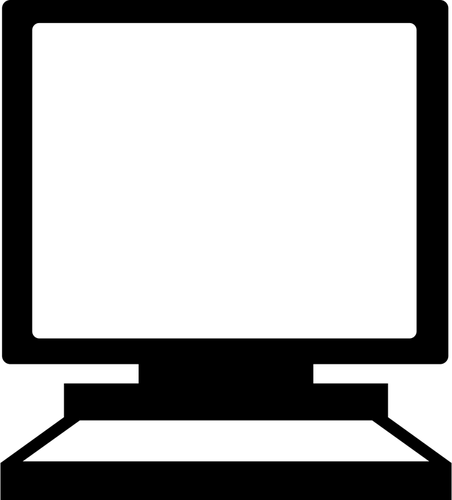
\includegraphics[width=\textwidth]{images/computer.png}};
		\draw [draw=black,fill=white] (-3.25,-0.5) rectangle ++(-3,1.5);
		\draw [draw=black,fill=white] (-3.75,0) rectangle ++(-3,1.5);
		\draw [draw=black,fill=white] (-4.25,0.5) rectangle ++(-3,1.5);
		\node[draw=none] at (-5.75,1.25) {Shard groups};
		\draw[<-] (-3,-0.3) -- (-2,-0.3);
		\draw[->] (-3,0) -- (-2,0);
		\node [cloud, draw, cloud puffs=10, cloud puff arc=120, aspect=2, inner ysep=1em, scale=1] {Internet};
	\end{tikzpicture}
	\caption{When a packet is sent from a node to the network, the receiving shard group can either set up a direct route to the Internet, or set up a route with an extra hop to some other external shard group. This adds an additional level of obfuscation to the communication.}
\end{figure}

\noindent To allow currently developed applications to join the network and promote adoption, the Unigrid daemon exposes a SOCKS5 proxy that allows the operating system and existing applications to connect to the network and communicate via it. Packets are routed through this SOCKS5 proxy and translated into communication packets that re-route communication onto the Unigrid network and into one of its \glspl{shardgroup}.

\pagebreak
\subsection{An encrypted in-memory FIFO blockchain}
\label{section:fifo}
To achieve a communication layer capable of high speeds with a reasonable latency penalty, the Unigrid network utilizes an in-memory FIFO blockchain. Blockchains in general have the ability to checksum data which allows for consensus and error correction perfect for real-time communication queues. Furthermore, a hashing function has been chosen where speed is preferred over collision resistance. Considering how fast the communication chains on the network need to progress, the choice of a slightly more naive hashing function should not cause any issues. Using the FNVJ64 hash function we can create a very rapidly moving blockchain.

\begin{figure}[H]
\centering
\begin{tikzpicture} 
	\begin{axis}[xbar,
		y axis line style = { opacity = 0 },
		axis x line = none,
		ytick = data,
		xmax = 6000,
		tickwidth = 0.05pt,
		enlarge y limits  = 0.15,
		enlarge x limits  = 0.005,
		title=Performance in megabytes per second (MB/s),
		symbolic y coords={SHA1, CRC32, Murmur3a, Murmur3f, FNVJ64},
		nodes near coords];
		\addplot[gray,fill] coordinates {(196,SHA1) (400,CRC32) (2130,Murmur3a) (3752,Murmur3f) (5879,FNVJ64)};
	\end{axis} 
\end{tikzpicture}
\caption{More naive hashing functions such as FNVJ64 offer a distinct performance advantage over more collision-resistant hash functions such as SHA-1. A rough estimation tells us that the performance increase is nearly 3000\% when compared to SHA-1, which can only achieve around 200 MB/s \cite{greenrobot} under the same hardware, in this specific example.}
\end{figure}

\noindent The \glspl{gridnode} on the network use the aforementioned hashing function to create a rapidly moving FIFO blockchain. When a \gls{gridnode} handles the communication for a node - that data is placed into the FIFO blockchain. Essentially, this means that each \gls{shardgroup} on the network  manages one or many small communication FIFO blockchains.

A communicating node will be grouped together with other nodes that are able to handle a similar bandwidth. When connecting, a node asks the network about \gls{shardgroup} information - asking which \glspl{shardgroup} might be willing to accept new communicating nodes. The node then connects to a given \gls{shardgroup} and starts accepting data from a FIFO blockchain. Whenever the node wants to access the public Internet, it populates the FIFO blockchain with a communication packet containing a fingerprint. This packet and the communication session is picked up by a \gls{gridnode} inside the \gls{shardgroup}. When the \gls{gridnode} answers, it answers by populating the FIFO blockchain with an answering packet containing the same fingerprint. Using this scheme, the two communicating nodes are able to find each other inside the Unigrid network - without knowing about each others physical location.

The in-memory FIFO blockchain works like a traditional FIFO queue but with the difference that each entry is hashed, while also containing the hash to the previous entry - just like a blockchain;

\begin{figure}[H]
\centering
\digraph[scale=0.8]{fifo}{
node [width=0.1, height=0.4 fontsize=10, rank=lr]
	nodesep=0.4;
	node [shape = box];
	{rank = same;A;B;C;D;E;F}

	A -> B -> C -> D -> E -> F
}
\caption{A very simplified subset of an in-memory FIFO blockchain queue. Packets are handled by the cluster in the order they are received into the queue. The queue is a "rolling" data structure that is flexible in size. Meaning that it can grow in size and queue up traffic more aggressively when the cluster can't keep up. Packets enter the queue on the left and exit it on the right, continuously updating the tail and head of the queue.}
\end{figure}

\section{Computing and storing data}
The Unigrid daemon and network aims for a sandboxed interpreter that takes advantage of The BNF Converter \cite{bnfc}, developed at the Centre for Language Technology at Chalmers University of Technology and The University of Gothenburg. The tool allows developers to define a language grammar in Backus-Naur-form, which is an extension based on the original paper by J.W Backus \cite{backus1959}. The converter generates a code template based on the language grammar provided and allows for the ability to rapidly write AST parsers and add logic for the grammar. In addition to this, the Unigrid daemon will parse binary web assembly.

These components should implement most of the WebAssembly specification \cite{webassembly}. Furthermore, the interpreter handles common operating system calls such as file operations and console operations and translate them to run on the Unigrid network. For example, a file operation writing file data, will instead redirect that operation onto the Unigrid network. Some time  ago, the official threads and atomics API \cite{webassemblythreads} was also completed and came out of alpha and beta status. In addition to this, the Unigrid network uses WebGPU for compute work that is intended to target GPU:s. The first public draft of WebGPU was recently published by W3C \cite{w3cwebgpu} and will allow the network to support this kind of workload as well - creating a truly universal low level solution.

Essentially, this creates a translation layer that, with a minimum amount of changes, will allow for the compilation and execution of a big portion of the current software base that exists. This eases adoption and makes it easier for developers and applications to transition to the Unigrid network.

\begin{figure}[H]
\centering
\digraph[scale=0.7]{jvmsandbox}{
node [width=0.2, height=0.5 fontsize=12, rank=lr]
	nodesep=0.3;

	subgraph cluster_3 {
		subgraph cluster_4 {
			style = filled;
			node [style=filled, color=white, shape=box, width=0.5] Interpreter
			label = "Sandbox";
			labelloc = b;
		}

		label = "Java Virtual Machine / GraalVM";
		labelloc = b;
	}

	"Compute chain" -> Interpreter
}
\caption{To protect the host \gls{gridnode} and achieve a high level of security and stability, the interpreter is implemented in Java and runs inside a sandboxed virtual machine. This means that most operating system access is limited or completely disabled in order to protect the underlying operating system environment of the \gls{gridnode}.}
\end{figure}

\section{Transaction data and duality consensus}
The original Unigrid implementation for handling transactions is based on Bitcoin and the work of Satoshi Nakamoto \cite{bitcoin2008}. With this design and consensus method, the time and effort needed to synchronize chain data rises as the size of the underlying blockchain increases. While it makes the data structure simpler and consensus easier to achieve, the design is rigid and wasteful, forcing participants to synchronize a lot of data that they have no direct relationship to. To address this issue, the Unigrid network will take advantage of its address tree ledger, as described in section \ref{section:delta}, to achieve a faster synchronization and a more segmented consensus method. Instead of storing every single transaction in a central ledger, the Unigrid network will, at the earliest convenience, separate this information into smaller blockchains where each wallet address tracked on the network governs exactly one blockchain.

To achieve consensus and data integrity a duality consensus method is employed. Whenever an address sends a transaction to another address, the network verifies that the two blockchains involved are in agreement and that all the nodes taking part in the consensus also agree. Rather than having to update and rely on an entire central ledger, two smaller blockchains can be updated, improving data sharing and synchronization times dramatically.

\section{Keeping the network updated}
The Unigrid network will continuously evolve, with frequent changes and new releases of the software for the network. Therefore, the traditional approach with members of the network manually updating their wallets and daemons is not feasible. It would create an additional turnaround time, where the foundation would have to wait long periods of time for the community to update before a new feature was enabled. Additionally, if the Unigrid network is deployed on hardware devices, such as routers, these need to be able to update on their own, without user-intervention.

The solution to this problem is to make the daemons and wallets react and check for new updates of the software. The Unigrid Foundation will control a private \emph{release} key. Whenever a new release is created and pushed to the network, the participants (or the current nodes) will try to sign this key with the public key provided with the software. If the key can be signed, they (the nodes) can assume the release is officially endorsed by The Unigrid Foundation.

Next, the \glspl{gridnode} on the network will have exactly one week to reject the release. If a \gls{gridnode} does not reject a release, the network will assume that the node in question accepts the new version. If a majority of the network accepts the new version, it will be applied by the network and all nodes on the network will update.

\pagebreak
\section{Future work}
This protocol and the algorithms discussed will evolve and change continuously as the Unigrid network, its protocol and related blockchains evolve and mature. Additional \gls{gridnode} sporks will be continuously defined, allowing the foundation and the community to manage and control the network. For example, a \gls{gridnode} spork with a value of ($1 > v > -1$) is being considered that would allow The Unigrid Foundation to quickly re-weight the planned reward implementation described in section \ref{section:dynreward}, if a situation arose where the network was unable to keep up with price changes of the underlying token.

The TOR network generates additional traffic, or noise, from the creation of its communication queues. Similarly, the Unigrid network will also generate extra traffic when clusters of nodes share and synchronize the encrypted in-memory FIFO blockchains. This property is what creates the obfuscation and makes the traffic untraceable. Future considerations and work will research how this particular way of creating anonymization can be optimized and how the networks should weight and organize participants and nodes in order to optimize network performance.

The current description of the address tree ledger is very general and only describes how the data structure will work - not how the data will be stored or indexed. The solution will require further research from The Unigrid Foundation. Developing a custom backend might be the only way to get the desired performance. At the same time, finding a usable third-party solution that gives acceptable performance could save some development time.

While the general structure and idea is the same, the dynamic \gls{gridnode} collateral adjustment, as described in section \ref{section:dyncol}, needs to be adjusted to account for any changes to the circulating token supply on the network. If the deployment stalls, The Unigrid Foundation can, based on the decision of the board, release additional tokens onto the market from its locked supply in order to fuel further adoption.

Supporting both binary web assembly and its text format might not be the most optimal solution at an early stage. More investigation is needed. An alternative could be to just implement the binary support initially.

Grouping of \glspl{gridnode} and how the selection of members should work needs to be investigated further. Most likely, we need an already deployed network to do live tests on in order to find optimal grouping strategies for \glspl{shardgroup}.

This work broadly describes select implementation details of the underlying network and how the foundation plans to implement some of the core functionality and algorithms. The specification and this paper will be divided into separate publications as the network develops and more detail is needed.

As defined by the statutes \cite{unigridstatutes} and charter \cite{unigridcharter} of the Unigrid Foundation - if any solution described in this paper or the current protocol is deemed inefficient or lacking in any way for an efficient operation of the network - the Unigrid Foundation and its developers will invest the necessary time, research and development needed to improve the network protocol and make the necessary changes to improve said solution or protocol.

\section{Conclusion}
We have clarified a solution to the deteriorating trend on the current network of the Internet and how it is possible for the increasing centralization and surveillance to be addressed using a multi-blockchain solution with an address tree ledger. The address ledger is a completely different approach to previous blockchain solutions and allows the network to quickly locate which specific blockchains different network nodes are part of and identify where data is located.

We have also shown how the Unigrid network is self-governing and how grouping and scoring of nodes is achieved on the network. The scoring, grouping and sharding of the network allows the topology of the network to adapt and get around areas of congestion. It has also been described how the sharding and grouping adds fault-tolerance and redundancy to data stored on the network.

The protocol solves the issue of an ever growing blockchain eventually reaching a size where it takes a very big amount of data to store or where it becomes nearly unusable, because the traversal of the data structures takes a lot of computational time. The original Bitcoin blockchain and the vast majority of other blockchain projects and cryptocurrencies have this bottleneck. The Unigrid network describes a solution that allows the network and its data to scale indefinitely. The reorganize functionality of the chains and the way that data is striped allows the data stored on the network to grow and even shrink in size.

Furthermore, we have demonstrated how the network runs distributed applications and deploys services that can never be interrupted by instability or outages, describing how the sandboxed translation layer on the \glspl{gridnode} interprets web assembly and web GPU into something that it can execute and run.

We have shown how the nodes on the network will govern themselves and update to new versions of the software when released by The Unigrid Foundation. We also explained why updates to the nodes need to be automated and how it benefits the network in the long term.

The work in this paper collects many proven principles and solutions and adapts them for use with a decentralized and distributed network solution. Some, like web assembly and web GPU, have recently been developed, while others have been used and proven in industry since many years back. Using the work in this paper, a robust and anonymous network capable of scaling indefinitely and handling enormous amounts of computation and storage will be developed.

\newpage
\section{License}
This paper is a continuous draft and should not be taken as an absolute description of the future state and implementation of the network. Rather, this paper will evolve together with the evolution of the network and the protocol. To preserve the historical work of the foundation, all public versions and the release history of this paper and its specifications will be published on the website of The Unigrid Foundation \cite{unigrid}.

Intermediate development releases should be called `draft versions`. When The Unigrid Foundation makes a formal and public release implementing the functionality as described in this paper, the paper should, together with that release of the network, be labelled as a `final version`.

The algorithms and descriptions covered herein may not be used to implement a separate implementation, network or product outside the oversight of The Unigrid Foundation. If any solution, product or network uses the algorithms or descriptions as described in this paper, in their own implementations, without the explicit permission of The Unigrid Foundation, the foundation has the right to seek compensation. As supported by the statutes of The Unigrid Foundation \cite{unigridstatutes}, the foundation does this to protect the integrity and stability of the Unigrid network, limiting network fragmentation and promoting the growth of an anonymous decentralized, global Internet that anyone can use and join.

In no event will The Unigrid Foundation be liable for any damages, including general, special, incidental or consequential damages arising out of the use, distribution or publication of this paper.

\clearpage

\begin{thebibliography}{999}

\bibitem{andy2017}
	Andy Klein, Backblaze,
	\emph{"Hard Drive Cost Per Gigabyte"},
	\href{https://www.backblaze.com/blog/hard-drive-cost-per-gigabyte}{www.backblaze.com},
	2017.

\bibitem{bitinfocharts2019}
	BitInfoCharts,
	\emph{"Cryptocurrency statistics, Blockchain Size"},
	\href{https://bitinfocharts.com}{bitinfocharts.com},
	\the\year{}.

\bibitem{facebook2018}
	Cale Weissman, Fast Company,
	\emph{"How Facebook Blew It"},
	\href{https://www.fastcompany.com/40550423/how-facebook-blew-it}{www.fastcompany.com},
	2018.

\bibitem{bnfc}
	Centre for Language Technology, Chalmers University of Technology and University of Gothenburg,
	\emph{"The BNF Converter"},
	\href{https://bnfc.digitalgrammars.com/}{bnfc.digitalgrammars.com}
	\the\year{}.

\bibitem{percival2006}
	Colin Percival, Wadham College, University of Oxford,
	\emph{"Matching with Mismatches and Assorted Applications"},
	\href{http://www.daemonology.net/papers/thesis.pdf}{www.daemonology.net},
	2006.

\bibitem{dashref2017}
	Dash Project,
	\emph{"Dash Developer Reference: Spork"},
	\href{https://dash-docs.github.io/en/developer-reference\%23spork}{dash-docs.github.io},
	2017-2019.

\bibitem{patterson1988}
	David A Patterson \& Garth Gibson \& Randy H Katz, University of California, Berkeley,
	\emph{"A Case for Redundant Arrays of Inexpensive Disks (RAID)"},
	\href{https://www.cs.cmu.edu/~garth/RAIDpaper/Patterson88.pdf}{www.cs.cmu.edu},
	1988.

\bibitem{darkcoin2014}
	Evan Duffield \& Kyle Hagan, The Darkcoin Developers,
	\emph{"Darkcoin: Peer­to­Peer Crypto­Currency with Anonymous Blockchain Transactions and an Improved Proof­of­Work System"},
	\href{https://dashpay.atlassian.net/wiki/download/attachments/132120878/Darkcoin\%20Whitepaper.pdf}{dashpay.atlassian.net},
	2014.

\bibitem{fips202}
	Federal Information Processing Standards,
	\emph{"SHA-3 STANDARD: PERMUTATION-BASED HASH AND EXTENDABLE OUTPUT FUNCTIONS"},
	\href{https://nvlpubs.nist.gov/nistpubs/FIPS/NIST.FIPS.202.pdf}{nvlpubs.nist.gov},
	2017.

\bibitem{greenrobot}
	Greenrobot Open Source Libraries,
	\emph{"Comparison of hash functions and performance benchmarks"},
	\href{https://greenrobot.org/essentials/features/performant-hash-functions-for-java/comparison-of-hash-functions}{greenrobot.org},
	\the\year{}.


\bibitem{53companies2018}
	Good Audience,
	\emph{"53 companies accepting cryptocurrency"},
	\href{https://blog.goodaudience.com/companies-accepting-cryptocurrency-4e224d72e25b}{blog.goodaudience.com},
	2018.

\bibitem{guardian2013}
	The Guardian,
	\emph{"NSA and GCHQ target Tor network that protects anonymity of web users"},
	\href{https://www.theguardian.com/world/2013/oct/04/nsa-gchq-attack-tor-network-encryption}{www.theguardian.com},
	2013.

\bibitem{igorparity2014}
	Igor Ostrovsky,
	\emph{"How RAID-6 dual parity calculation works"}
	\href{https://igoro.com/archive/how-raid-6-dual-parity-calculation-works/}{igoro.com},
	2014.

\bibitem{japan2017}
	Japanese Financial Services Agency,
	\emph{"About result of public comment for 'government orders to revise a part of the banking law enforcement order (draft)'"},
	\href{https://www.fsa.go.jp/news/28/ginkou/20170324-1.html}{www.fsa.go.jp},
	2017.

\bibitem{backus1959}
	J. W. Backus,
	\emph{"The Syntax and Semantics of the Proposed International Algebraic Language of the Zurich ACM-GAMM Conference. Proceedings of the International Conference on Information Processing"}
	\href{http://www.softwarepreservation.org/projects/ALGOL/paper/Backus-Syntax_and_Semantics_of_Proposed_IAL.pdf}{www.softwarepreservation.org},
	1959.

\bibitem{chen1990}
	Peter M. Chen \& David A Patterson, University of California, Berkeley,
	\emph{"Maximizing Performance in a Striped Disk Array"},
	\href{http://web.eecs.umich.edu/~pmchen/Rio/papers/chen90_1.pdf}{web.eecs.umich.edu},
	1990.

\bibitem{pivxrepo}
	The PIVX Team,
	\emph{"PIVX Core integration/staging repository"},
	\href{https://github.com/PIVX-Project/PIVX}{www.github.com},
	\the\year{}.

\bibitem{guardian2017}
	Rajeev Syal \& Denis Campbell, The Guardian,
	\emph{"NHS data loss scandal deepens with further 162,000 files missing"},
	\href{https://www.theguardian.com/society/2017/oct/16/nhs-data-loss-scandal-deepens-with-162000-more-files-missing}{www.theguardian.com},
	2017.

\bibitem{bitcoin2008}
	Satoshi Nakamoto,
	\emph{"Bitcoin: A Peer-to-Peer Electronic Cash System"},
	\href{http://www.bitcoin.org}{www.bitcoin.org},
	2008.

\bibitem{lz42017}
	Se-Jun Kwon, Sang-Hoon Kim, Hyeong-Jun Kim, and Jin-Soo Kim, College of Information and Communication Engineering, Sungkyunkwan University,
	\emph{"LZ4m: A Fast Compression Algorithm for In-Memory Data"},
	\href{http://csl.skku.edu/papers/icce17.pdf}{csl.skku.edu},
	2017.

\bibitem{songze2018}
	Songze Li, Mingchao Yu, A. Salman Avestimehr, Sreeram Kannan \& Pramod Viswanath, University of Southern California, University of Washington \& University of Illinois at Urbana-Champaign,
	\emph{"PolyShard: Coded Sharding Achieves Linearly Scaling Efficiency and Security Simultaneously"},
	\href{https://arxiv.org/pdf/1809.10361.pdf}{arxiv.org},
	2018.

\bibitem{sothe2018}
	Sothearath Seang, Dominique Torre,
	\emph{"Proof of Work and Proof of Stake consensus protocols: a blockchain application for local complementary currencies"},
	\href{https://gdre-scpo-aix.sciencesconf.org/195470/document}{gdre-scpo-aix.sciencesconf.org},
	2018.

\bibitem{ekrona2019}
	The Swedish Riksbank,
	\emph{"E-krona"},
	\href{https://www.riksbank.se/en-gb/payments--cash/e-krona}{www.riksbank.se},
	2019.

\bibitem{tor2021}
	The Tor Project, Inc,
	\emph{Defend yourself against tracking and surveillance. Circumvent censorship},
	\href{https://www.torproject.org}{www.torproject.org},
	\the\year{}.

\bibitem{unigridcharter}
	The Unigrid Foundation,
	\emph{"The Unigrid Foundation Charter"},
	\href{https://www.unigrid.org/link-not-yet-available}{www.unigrid.org},
	\the\year{}.

\bibitem{unigridstatutes}
	The Unigrid Foundation,
	\emph{"The Unigrid Foundation Statutes"},
	\href{https://www.unigrid.org/link-not-yet-available}{www.unigrid.org},
	\the\year{}.

\bibitem{unigrid}
	The Unigrid Foundation,
	\emph{"The Unigrid Foundation Website \& Project Page"},
	\href{https://www.unigrid.org}{www.unigrid.org},
	\the\year{}.

\bibitem{webassemblythreads}
	WebAssembly Community Group,
	\emph{"Threads Proposal for WebAssembly"},
	\href{https://github.com/WebAssembly/threads}{github.com},
	\the\year{}.

\bibitem{webassembly}
	WebAssembly Community Group,
	\emph{"WebAssembly Specification"},
	\href{https://webassembly.github.io/spec/core/_download/WebAssembly.pdf}{webassembly.github.io},
	\the\year{}.

\bibitem{w3cwebgpu}
	W3C,
	\emph{"WebGPU, W3C First Public Working Draft, 18 May 2021"},
	\href{https://www.w3.org/TR/2021/WD-webgpu-20210518/}{www.w3.org},
	2021.

\bibitem{finitefield2021}
	Wikipedia,
	\emph{"Finite field arithmetic"},
	\href{https://en.wikipedia.org/wiki/Finite_field_arithmetic}{en.wikipedia.org},
	\the\year{}.

\bibitem{historybitcoin2019}
	Wikipedia,
	\emph{"History of Bitcoin"},
	\href{https://en.wikipedia.org/wiki/History_of_bitcoin}{en.wikipedia.org},
	\the\year{}.

\bibitem{historyinternet2019}
	Wikipedia,
	\emph{"History of the Internet"},
	\href{https://en.wikipedia.org/wiki/History_of_the_Internet}{en.wikipedia.org},
	\the\year{}.

\end{thebibliography}

\clearpage
\printglossaries

\end{document}
